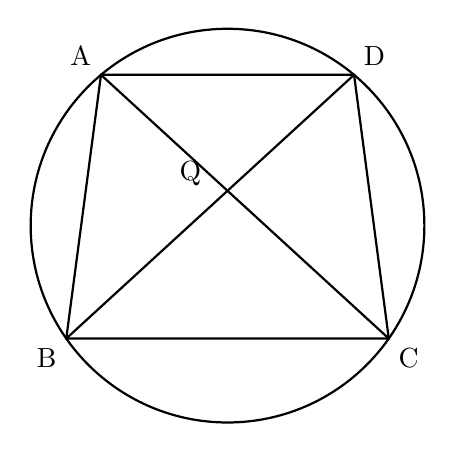
\begin{tikzpicture}[scale=1]

    % Define the radius of the circle
    \def\R{2.5}

    % Define coordinates for the points on the circle to match the proportions in the image
    % A and D are closer to the top, B and C are wider at the bottom
    \coordinate (A) at (130:\R);
    \coordinate (D) at (50:\R);
    \coordinate (B) at (215:\R);
    \coordinate (C) at (325:\R);

    % Draw the circle
    \draw[thick] (0,0) circle (\R);

    % Draw the inscribed quadrilateral ABCD
    \draw[thick] (A) -- (B) -- (C) -- (D) -- cycle;

    % Draw the diagonal segments AC and BD
    \draw[thick] (A) -- (C);
    \draw[thick] (B) -- (D);

    % Calculate the intersection point Q of the diagonals
    \coordinate (Q) at (intersection of A--C and B--D);

    % Place the labels for the vertices exactly as shown in the image
    \node[above left] at (A) {A};
    \node[above right] at (D) {D};
    \node[below left] at (B) {B};
    \node[below right] at (C) {C};

    % Label Q is positioned slightly to the top-left of the intersection point
    % Moved further left by changing xshift from -2pt to -6pt
    \node[left, xshift=-6pt, yshift=6pt] at (Q) {Q};

\end{tikzpicture}